% PART 4 (SECTION 8.4)
\part{Section 8.4}
%%%%%%%%%%%%%%%%%%%%%%%%%%%%%%%%%%%%%%%
\begin{transitionframe}
    \begin{center}
    { 
        \Huge \textcolor{white}{\textbf{Volume and Surface Area}}
        \\[-1em]
        \noindent\textcolor{white}{\rule{12cm}{0.4pt}}
        
        %\large \textcolor{white}{Section 8.4}
    }
    \end{center}
\end{transitionframe}
%%%%%%%%%%%%%%%%%%%%%%%%%%%%%%%%%%%%%%%
%        SLIDE 
%%%%%%%%%%%%%%%%%%%%%%%%%%%%%%%%%%%%%%%
\begin{frame}{Outline}
    \begin{columns}[t]
        \begin{column}{.5\textwidth}
            \tableofcontents[part=4, sections={1-2}]
        \end{column}
        \begin{column}{.5\textwidth}
            \tableofcontents[part=4, sections={3-4}]
        \end{column}
    \end{columns}
\end{frame}
%%%%%%%%%%%%%%%%%%%%%%%%%%%%%%%%%%%%%%%
%        SLIDE 
%%%%%%%%%%%%%%%%%%%%%%%%%%%%%%%%%%%%%%%
\section{Polyhedra}
\subsection{What is Polyhedra?}
\begin{frame}{Polyhedra}
    \begin{itemize}
        \item A polyhedron (plural polyhedra) is closed figure formed by a number of polygons.
    \end{itemize}
    %
    \begin{block}{Definition}
        A polyhedron must meet 3 conditions:
        \begin{itemize}
            \item closed figure
            \item created by straight lines only
            \item 3-Dimensional object
        \end{itemize}
    \end{block}
    %
    \begin{figure}[H]
        \centering
        % DEFINING COLORS COF, PUR, GREEO AND GREET
\definecolor{cof}{RGB}{219,144,71}
\definecolor{pur}{RGB}{186,146,162}
\definecolor{greeo}{RGB}{91,173,69}
\definecolor{greet}{RGB}{52,111,72}
% TETRAHEDRON
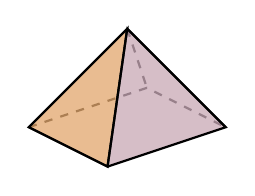
\begin{tikzpicture}[thick,scale=2.5]
    \coordinate (A1) at (0,0);
    \coordinate (A2) at (0.6,0.2);
    \coordinate (A3) at (1,0);
    \coordinate (A4) at (0.4,-0.2);
    \coordinate (B1) at (0.5,0.5);
    %
    \begin{scope}[thick,dashed,,opacity=0.6]
        \draw (A1) -- (A2) -- (A3);
        \draw (B1) -- (A2);
    \end{scope}
    \draw[fill=cof,opacity=0.6] (A1) -- (A4) -- (B1);
    \draw[fill=pur,opacity=0.6] (A4) -- (B1) -- (A3);
    %
    \draw (A1) -- (B1) -- (A4) --cycle;
    \draw (A4) -- (A3) -- (B1) ;
    %
\end{tikzpicture}
% RECTANGULAR CUBE
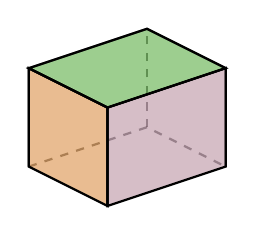
\begin{tikzpicture}[thick,scale=2.5]
    \coordinate (A1) at (0,0);
    \coordinate (A2) at (0.6,0.2);
    \coordinate (A3) at (1,0);
    \coordinate (A4) at (0.4,-0.2);
    \coordinate (B1) at (0,0.5);
    \coordinate (B2) at (0.6,0.7);
    \coordinate (B3) at (1,0.5);
    \coordinate (B4) at (0.4,0.3);
    %
    \begin{scope}[thick,dashed,,opacity=0.6]
        \draw (A1) -- (A2) -- (A3);
        \draw (A2) -- (B2);
    \end{scope}
    %
    \draw[fill=cof,opacity=0.6] (A1) -- (B1) -- (B4) -- (A4);
    \draw[fill=pur,opacity=0.6] (A4) -- (B4) -- (B3) -- (A3);
    \draw[fill=greeo,opacity=0.6] (B4) -- (B1) -- (B2) -- (B3);
    %
    \draw (A1) -- (B1) -- (B4) -- (A4) --cycle;
    \draw (A4) -- (B4) -- (B3) -- (A3) --cycle;
    \draw (B4) -- (B1) -- (B2) -- (B3) --cycle;
    %
\end{tikzpicture}
% OCTAHEDRON
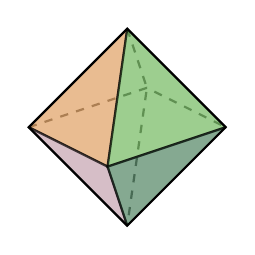
\begin{tikzpicture}[thick,scale=2.5]
    \coordinate (A1) at (0,0);
    \coordinate (A2) at (0.6,0.2);
    \coordinate (A3) at (1,0);
    \coordinate (A4) at (0.4,-0.2);
    \coordinate (B1) at (0.5,0.5);
    \coordinate (B2) at (0.5,-0.5);
    %
    \begin{scope}[thick,dashed,,opacity=0.6]
        \draw (A1) -- (A2) -- (A3);
        \draw (B1) -- (A2) -- (B2);
    \end{scope}
    %
    \draw[fill=cof,opacity=0.6] (A1) -- (A4) -- (B1);
    \draw[fill=pur,opacity=0.6] (A1) -- (A4) -- (B2);
    \draw[fill=greeo,opacity=0.6] (A3) -- (A4) -- (B1);
    \draw[fill=greet,opacity=0.6] (A3) -- (A4) -- (B2);
    \draw (B1) -- (A1) -- (B2) -- (A3) --cycle;
\end{tikzpicture}
% Prism
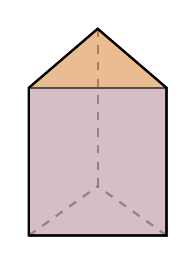
\begin{tikzpicture}[thick,scale=2.5]
    \coordinate (A1) at (0,0);
    \coordinate (A3) at (0.7,0);
    \coordinate (A4) at (0,-0.75);
    \coordinate (A5) at (0.7,-0.75);
    \coordinate (B1) at (0.35,0.3);
    \coordinate (B2) at (0.35,-0.5);
    %
    \begin{scope}[thick,dashed,opacity=0.6]
        \draw (B1)  -- (B2);
        \draw (A4) -- (B2);
        \draw (A5) -- (B2);
    \end{scope}
    %
    \draw[fill=cof,opacity=0.6] (A1) -- (B1) -- (A3);
    \draw[fill=pur,opacity=0.6] (A1) -- (A3) -- (A5) -- (A4);
    %
    \draw (A1) -- (B1) -- (A3) -- (A5) -- (A4) --cycle;
    %
\end{tikzpicture}
    \end{figure}
\end{frame}
%%%%%%%%%%%%%%%%%%%%%%%%%%%%%%%%%%%%%%%
%        SLIDE 
%%%%%%%%%%%%%%%%%%%%%%%%%%%%%%%%%%%%%%%
\subsection{Faces, Vertices, and Edges}
\begin{frame}{Faces, Vertices, and Edges}
    \begin{itemize}
        \item \textbf{Face}: Each flat surface (or each polygon).
        \item \textbf{Vertex}: Corners of faces.
        \item \textbf{Edge}: A line segment between two faces.
    \end{itemize}
    %
    \begin{figure}[H]
        \centering
        

\tikzset{every picture/.style={line width=0.75pt}} %set default line width to 0.75pt        

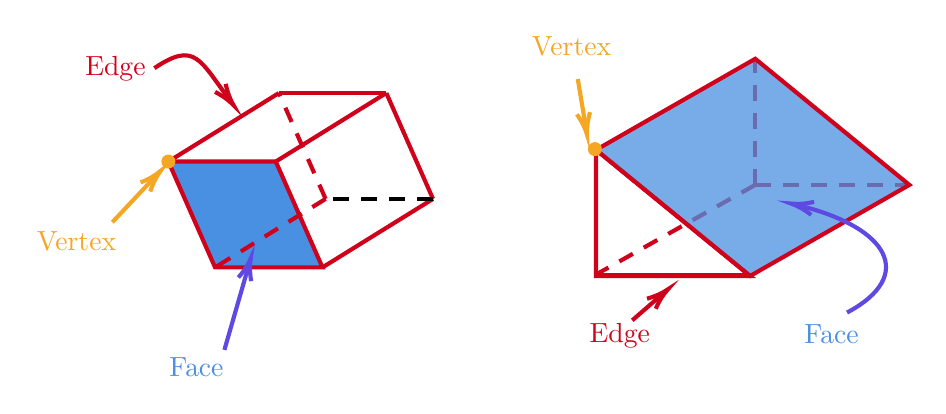
\begin{tikzpicture}[x=0.75pt,y=0.75pt,yscale=-1,xscale=1, scale= 0.75]
%uncomment if require: \path (0,288); %set diagram left start at 0, and has height of 288

%Shape: Rectangle [id:dp053370527561274805] 
\draw  [color={rgb, 255:red, 208; green, 2; blue, 27 }  ,draw opacity=1 ][fill={rgb, 255:red, 74; green, 144; blue, 226 }  ,fill opacity=1 ][line width=1.5]  (130,96) -- (199,96) -- (229,164) -- (160,164) -- cycle ;
%Straight Lines [id:da7233344038492684] 
\draw [color={rgb, 255:red, 208; green, 2; blue, 27 }  ,draw opacity=1 ][line width=1.5]    (199,96) -- (270,52) ;


%Straight Lines [id:da8870385695360932] 
\draw [color={rgb, 255:red, 208; green, 2; blue, 27 }  ,draw opacity=1 ][line width=1.5]    (130,96) -- (201,52) ;


%Straight Lines [id:da6880167264201218] 
\draw [color={rgb, 255:red, 208; green, 2; blue, 27 }  ,draw opacity=1 ][line width=1.5]    (229,164) -- (300,120) ;


%Straight Lines [id:da8629284451428976] 
\draw [color={rgb, 255:red, 208; green, 2; blue, 27 }  ,draw opacity=1 ][line width=1.5]    (300,120) -- (270,52) ;


%Straight Lines [id:da5801797655392487] 
\draw [color={rgb, 255:red, 208; green, 2; blue, 27 }  ,draw opacity=1 ][line width=1.5]    (270,52) -- (201,52) ;


%Straight Lines [id:da33437733704095596] 
\draw [color={rgb, 255:red, 208; green, 2; blue, 27 }  ,draw opacity=1 ][line width=1.5]  [dash pattern={on 5.63pt off 4.5pt}]  (231,120) -- (201,52) ;


%Straight Lines [id:da7324938230911522] 
\draw [line width=1.5]  [dash pattern={on 5.63pt off 4.5pt}]  (300,120) -- (231,120) ;


%Straight Lines [id:da04595951918657737] 
\draw [color={rgb, 255:red, 208; green, 2; blue, 27 }  ,draw opacity=1 ][line width=1.5]  [dash pattern={on 5.63pt off 4.5pt}]  (231,120) -- (160,164) ;


%Shape: Right Triangle [id:dp15828119672901897] 
\draw  [color={rgb, 255:red, 208; green, 2; blue, 27 }  ,draw opacity=1 ][line width=1.5]  (404.75,88.5) -- (503.75,169.5) -- (404.75,169.5) -- cycle ;
%Straight Lines [id:da18371357143649392] 
\draw [color={rgb, 255:red, 208; green, 2; blue, 27 }  ,draw opacity=1 ][line width=1.5]  [dash pattern={on 5.63pt off 4.5pt}]  (507,111) -- (507,30) ;


%Straight Lines [id:da5323303129683379] 
\draw [color={rgb, 255:red, 208; green, 2; blue, 27 }  ,draw opacity=1 ][line width=1.5]  [dash pattern={on 5.63pt off 4.5pt}]  (507,111) -- (606,111) ;


%Straight Lines [id:da1934412072495324] 
\draw [color={rgb, 255:red, 208; green, 2; blue, 27 }  ,draw opacity=1 ][line width=1.5]  [dash pattern={on 5.63pt off 4.5pt}]  (404,169) -- (507,111) ;


%Curve Lines [id:da9915257466456324] 
\draw [color={rgb, 255:red, 208; green, 2; blue, 27 }  ,draw opacity=1 ][line width=1.5]    (121,36) .. controls (147.33,18.45) and (149.88,30.37) .. (170.39,57.86) ;
\draw [shift={(172,60)}, rotate = 232.82] [color={rgb, 255:red, 208; green, 2; blue, 27 }  ,draw opacity=1 ][line width=1.5]    (14.21,-4.28) .. controls (9.04,-1.82) and (4.3,-0.39) .. (0,0) .. controls (4.3,0.39) and (9.04,1.82) .. (14.21,4.28)   ;

%Shape: Circle [id:dp6348766282723517] 
\draw  [draw opacity=0][fill={rgb, 255:red, 245; green, 166; blue, 35 }  ,fill opacity=1 ] (125.5,96) .. controls (125.5,93.51) and (127.51,91.5) .. (130,91.5) .. controls (132.49,91.5) and (134.5,93.51) .. (134.5,96) .. controls (134.5,98.49) and (132.49,100.5) .. (130,100.5) .. controls (127.51,100.5) and (125.5,98.49) .. (125.5,96) -- cycle ;
%Straight Lines [id:da9603817642462407] 
\draw [color={rgb, 255:red, 245; green, 166; blue, 35 }  ,draw opacity=1 ][line width=1.5]    (94,135) -- (122.95,104.19) ;
\draw [shift={(125,102)}, rotate = 493.21] [color={rgb, 255:red, 245; green, 166; blue, 35 }  ,draw opacity=1 ][line width=1.5]    (14.21,-4.28) .. controls (9.04,-1.82) and (4.3,-0.39) .. (0,0) .. controls (4.3,0.39) and (9.04,1.82) .. (14.21,4.28)   ;

%Straight Lines [id:da6450171763852104] 
\draw [color={rgb, 255:red, 94; green, 74; blue, 226 }  ,draw opacity=1 ][line width=1.5]    (166,217) -- (182.17,160.88) ;
\draw [shift={(183,158)}, rotate = 466.07] [color={rgb, 255:red, 94; green, 74; blue, 226 }  ,draw opacity=1 ][line width=1.5]    (14.21,-4.28) .. controls (9.04,-1.82) and (4.3,-0.39) .. (0,0) .. controls (4.3,0.39) and (9.04,1.82) .. (14.21,4.28)   ;

%Shape: Polygon [id:ds14971897219625419] 
\draw  [color={rgb, 255:red, 208; green, 2; blue, 27 }  ,draw opacity=1 ][fill={rgb, 255:red, 74; green, 144; blue, 226 }  ,fill opacity=0.75 ][line width=1.5]  (507,30) -- (606,111) -- (503.75,169.5) -- (404.75,88.5) -- cycle ;
%Straight Lines [id:da1871099492645416] 
\draw [color={rgb, 255:red, 208; green, 2; blue, 27 }  ,draw opacity=1 ][line width=1.5]    (503,169) -- (404,169) ;


%Straight Lines [id:da5598317572787015] 
\draw [color={rgb, 255:red, 208; green, 2; blue, 27 }  ,draw opacity=1 ][line width=1.5]    (428,198) -- (448.74,179.97) ;
\draw [shift={(451,178)}, rotate = 498.99] [color={rgb, 255:red, 208; green, 2; blue, 27 }  ,draw opacity=1 ][line width=1.5]    (14.21,-4.28) .. controls (9.04,-1.82) and (4.3,-0.39) .. (0,0) .. controls (4.3,0.39) and (9.04,1.82) .. (14.21,4.28)   ;

%Shape: Circle [id:dp5936650276871587] 
\draw  [draw opacity=0][fill={rgb, 255:red, 245; green, 166; blue, 35 }  ,fill opacity=1 ] (399.5,88) .. controls (399.5,85.51) and (401.51,83.5) .. (404,83.5) .. controls (406.49,83.5) and (408.5,85.51) .. (408.5,88) .. controls (408.5,90.49) and (406.49,92.5) .. (404,92.5) .. controls (401.51,92.5) and (399.5,90.49) .. (399.5,88) -- cycle ;
%Straight Lines [id:da46178057371883363] 
\draw [color={rgb, 255:red, 245; green, 166; blue, 35 }  ,draw opacity=1 ][line width=1.5]    (393,43) -- (398.51,76.04) ;
\draw [shift={(399,79)}, rotate = 260.54] [color={rgb, 255:red, 245; green, 166; blue, 35 }  ,draw opacity=1 ][line width=1.5]    (14.21,-4.28) .. controls (9.04,-1.82) and (4.3,-0.39) .. (0,0) .. controls (4.3,0.39) and (9.04,1.82) .. (14.21,4.28)   ;

%Curve Lines [id:da39173533566192775] 
\draw [color={rgb, 255:red, 94; green, 74; blue, 226 }  ,draw opacity=1 ][line width=1.5]    (566,193) .. controls (610.33,169.36) and (593.53,137.96) .. (532.8,123.64) ;
\draw [shift={(530,123)}, rotate = 372.53] [color={rgb, 255:red, 94; green, 74; blue, 226 }  ,draw opacity=1 ][line width=1.5]    (14.21,-4.28) .. controls (9.04,-1.82) and (4.3,-0.39) .. (0,0) .. controls (4.3,0.39) and (9.04,1.82) .. (14.21,4.28)   ;


% Text Node
\draw (96,36) node  [align=left] {\textcolor[rgb]{0.82,0.01,0.11}{Edge}};
% Text Node
\draw (71,147) node  [align=left] {\textcolor[rgb]{0.96,0.65,0.14}{Vertex}};
% Text Node
\draw (148,228) node [color={rgb, 255:red, 74; green, 144; blue, 226 }  ,opacity=1 ] [align=left] {\textcolor[rgb]{0.29,0.56,0.89}{Face}};
% Text Node
\draw (420,208) node  [align=left] {\textcolor[rgb]{0.82,0.01,0.11}{Edge}};
% Text Node
\draw (556,207) node [color={rgb, 255:red, 74; green, 144; blue, 226 }  ,opacity=1 ] [align=left] {\textcolor[rgb]{0.29,0.56,0.89}{Face}};
% Text Node
\draw (389,22) node  [align=left] {\textcolor[rgb]{0.96,0.65,0.14}{Vertex}};
% % Text Node
% \draw (198,268) node   {$( a)$};
% % Text Node
% \draw (485,268) node   {$( b)$};


\end{tikzpicture}
    \end{figure}
\end{frame}
%%%%%%%%%%%%%%%%%%%%%%%%%%%%%%%%%%%%%%%
%        SLIDE 
%%%%%%%%%%%%%%%%%%%%%%%%%%%%%%%%%%%%%%%
\subsection{Euler's Polyhedron Formula}
\begin{frame}[t]{Euler's Polyhedron Formula}
    \begin{columns}[c]
        \column{0.45\textwidth}
        %
        \begin{itemize}
            \item Leonhard Euler was a Swiss mathematician who made enormous contributions to a wide range of fields in mathematics.
            \item Euler discovered a relation between number of vertices, number of faces, and number of edges.
        \end{itemize}
        %
        \begin{block}{Euler's Formula}
             Let $V$ be the number of vertices, $E$ be the number of edges and $F$ be the number of faces of a polyhedon. Then
             \[ V-E+F=2 \]
        \end{block}
        %***** 2nd column *****
        \column{0.45\textwidth}    
        %
        \begin{figure}[H]
            \centering
            \includegraphics[width=0.6\textwidth]{pics/Leonhard_Euler.jpg}
            \caption*{Leonhard Euler (1707-1783)}
        \end{figure}
        % \begin{figure}[H]
        %     \centering
        %     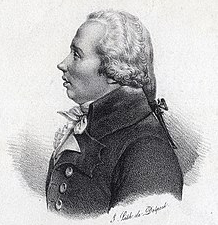
\includegraphics[width=0.35\textwidth]{pics/legendre.png}
        % \end{figure}
        % \begin{itemize}
        %     \item Euler mentioned his result in a letter to Goldbach in 1750. However he did not give the first correct proof of his formula.
        %     \item French mathematician Adrian Marie Legendre (1752-1833) was the first to prove using Spherical Geometry.
        % \end{itemize}
    \end{columns}

\end{frame}
%%%%%%%%%%%%%%%%%%%%%%%%%%%%%%%%%%%%%%%
%        SLIDE 
%%%%%%%%%%%%%%%%%%%%%%%%%%%%%%%%%%%%%%%
\begin{frame}{Euler's Polyhedron Formula (Cont'd)}
    \textbf{Examples}:
    %
    \begin{columns}
    %
    \column{0.25\textwidth}
    \begin{figure}[H]
        \centering
        % DEFINING COLORS COF, PUR, GREEO AND GREET
\definecolor{cof}{RGB}{219,144,71}
\definecolor{pur}{RGB}{186,146,162}
\definecolor{greeo}{RGB}{91,173,69}
\definecolor{greet}{RGB}{52,111,72}
% CUBE
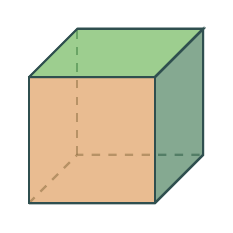
\begin{tikzpicture}[thick,scale=0.8,DarkSlateGray]
    \coordinate (A1) at (-1,-1,-1);
    \coordinate (A2) at (-1,-1,1);
    \coordinate (A3) at (-1,1,-1);
    \coordinate (A4) at (-1,1,1);
    \coordinate (B1) at (1,-1,-1);
    \coordinate (B2) at (1,-1,1);
    \coordinate (B3) at (1,1,-1);
    \coordinate (B4) at (1,1,1);
    %
    % Drawing dashed lines
    \begin{scope}[thick,dashed,opacity=0.6]
        \draw (A2) -- (A1) -- (B1);
        \draw (A1) -- (A3);
    \end{scope}
    %
    % Color Faces
    \draw[fill=cof,opacity=0.6]   (A4) -- (B4) -- (B2) -- (A2) ;
    \draw[fill=greet,opacity=0.6]   (B4) -- (B3) -- (B1) -- (B2) ;
    \draw[fill=greeo,opacity=0.6] (A4) -- (B4) -- (B3) -- (A3) ;
    %
    % Drawing Edges
    \draw (A2) -- (B2) -- (B1) ;
    \draw (A2) -- (A4) -- (B4) -- (B2) -- cycle ;
    \draw (A4) -- (A3) -- (B3) -- (B4) ;   
    \draw (B3) -- (B1);
    %
\end{tikzpicture}
    \end{figure}
    %
    \begin{center}
        Cube
    \end{center}
    %
    \begin{align*}
        & V=8,\; E=12,\; F=6
        \\
        &V-E+F = 2\ \checkmark
    \end{align*}   
    %
    \column{0.33\textwidth}
    \begin{figure}[H]
        \centering
        % DEFINING COLORS COF, PUR, GREEO AND GREET
\definecolor{cof}{RGB}{219,144,71}
\definecolor{pur}{RGB}{186,146,162}
\definecolor{greeo}{RGB}{91,173,69}
\definecolor{greet}{RGB}{52,111,72}
% Icosphedron
    \tdplotsetmaincoords{60}{100}
    \begin{tikzpicture}[tdplot_main_coords,scale=1,line join=round, scale=0.4]
    \pgfmathsetmacro\a{2}
    \pgfmathsetmacro{\phi}{\a*(1+sqrt(5))/2}
    \path 
    coordinate(A) at (0,\phi,\a)
    coordinate(B) at (0,\phi,-\a)
    coordinate(C) at (0,-\phi,\a)
    coordinate(D) at (0,-\phi,-\a)
    coordinate(E) at (\a,0,\phi)
    coordinate(F) at (\a,0,-\phi)
    coordinate(G) at (-\a,0,\phi)
    coordinate(H) at (-\a,0,-\phi)
    coordinate(I) at (\phi,\a,0)
    coordinate(J) at (\phi,-\a,0)
    coordinate(K) at (-\phi,\a,0)
    coordinate(L) at (-\phi,-\a,0); 
    \draw[dashed, thick]    (B) -- (H) -- (F) 
    (D) -- (L) -- (H) --cycle 
    (K) -- (L) -- (H) --cycle
    (K) -- (L) -- (G) --cycle
    (C) -- (L) (B)--(K) (A)--(K)
    ;

        \draw[thick]
        (A) -- (I) -- (B) --cycle 
        (F) -- (I) -- (B) --cycle 
        (F) -- (I) -- (J) --cycle
        (F) -- (D) -- (J) --cycle
        (C) -- (D) -- (J) --cycle
        (C) -- (E) -- (J) --cycle
        (I) -- (E) -- (J) --cycle
        (I) -- (E) -- (A) --cycle
        (G) -- (E) -- (A) --cycle
        (G) -- (E) -- (C) --cycle
        ; 
        \draw[fill=DarkSeaGreen,opacity=0.6] (A) -- (I) -- (B) --cycle ;
        \draw[fill=DarkKhaki,opacity=0.6]  (F) -- (I) -- (B) --cycle ;
        \draw[fill=Tan,opacity=0.6]  (F) -- (I) -- (J) --cycle;
        \draw[fill=CadetBlue,opacity=0.6]  (F) -- (D) -- (J) --cycle;
        \draw[fill=LightYellow,opacity=0.6]    (C) -- (D) -- (J) --cycle;
        \draw[fill=Thistle,opacity=0.6]   (C) -- (E) -- (J) --cycle;
        \draw[fill=DarkGray,opacity=0.6]  (I) -- (E) -- (J) --cycle;
        \draw[fill=LightSteelBlue,opacity=0.6]     (I) -- (E) -- (A) --cycle;
        \draw[fill=DarkSalmon,opacity=0.6]   (G) -- (E) -- (A) --cycle;
        \draw[fill=LightPink,opacity=0.6]    (G) -- (E) -- (C) --cycle;
\end{tikzpicture}
    \end{figure}   
    %
    \begin{center}
        Icosahedron 
    \end{center}
    %
    %
    \begin{align*}
        & V=12,\; E=30,\; F=20
        \\
        &V-E+F = 2\ \checkmark
    \end{align*}   
    %
    \end{columns}
\end{frame}
%%%%%%%%%%%%%%%%%%%%%%%%%%%%%%%%%%%%%%%
%        SLIDE 
%%%%%%%%%%%%%%%%%%%%%%%%%%%%%%%%%%%%%%%
\begin{frame}[t]{Example (Does this shape exist?)}
    \begin{example}
        Do the following shapes exist?
        \begin{enumerate}[(a)]
            \item A polyhedron with $V=10$, $E=22$, and $F=14$
            \item A polyhedron with $V= 14$, $E=21$, and $F= 10$
        \end{enumerate}
    \end{example}
\end{frame}
%%%%%%%%%%%%%%%%%%%%%%%%%%%%%%%%%%%%%%%
%        SLIDE 
%%%%%%%%%%%%%%%%%%%%%%%%%%%%%%%%%%%%%%%
\begin{frame}[t]{Example (Euler's Formula)}
    \begin{example}
        A certain polyhedron has 16 vertices and 10 faces. Determine the number of edges on the polyhedron.
    \end{example}
\end{frame}
%%%%%%%%%%%%%%%%%%%%%%%%%%%%%%%%%%%%%%%
%        SLIDE 
%%%%%%%%%%%%%%%%%%%%%%%%%%%%%%%%%%%%%%%
\section{Types of Polyhedra}
\begin{frame}[t]{Types of Polyhedra}
    \begin{figure}[h]
        \centering
        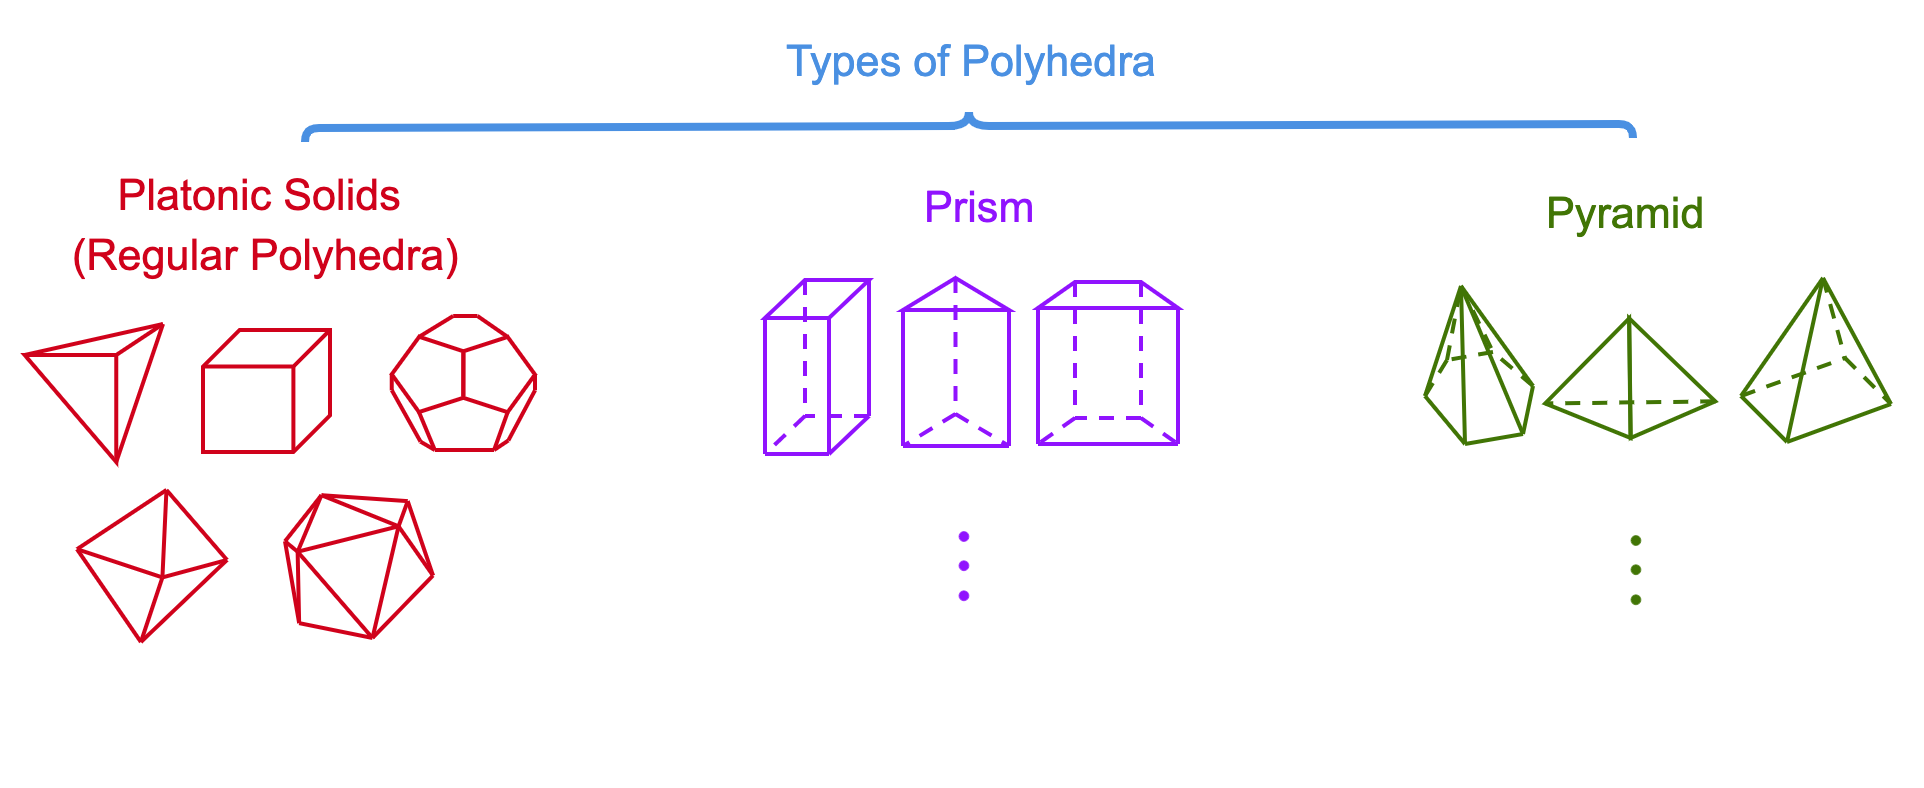
\includegraphics[scale=0.22]{pics/types_polyhedra.png}
    \end{figure}
\end{frame}
%%%%%%%%%%%%%%%%%%%%%%%%%%%%%%%%%%%%%%%
%        SLIDE 
%%%%%%%%%%%%%%%%%%%%%%%%%%%%%%%%%%%%%%%
\subsection{Platonic Solids}
\begin{frame}[t]{Platonic Solids}
    %
    \begin{itemize}
        \item All faces are \textbf{regular} polygons of the same size and shape.
        \item There are only 5 platonic solids (why? watch this video from \hyperlink{http://www.youtube.com/watch?v=gVzu1_12FUc}{\textcolor{blue}{\underline{Numberphile}}}).
    \end{itemize}
    %
    \begin{figure}[H]
        \centering
        % DEFINING COLORS COF, PUR, GREEO AND GREET
\definecolor{cof}{RGB}{219,144,71}
\definecolor{pur}{RGB}{186,146,162}
\definecolor{greeo}{RGB}{91,173,69}
\definecolor{greet}{RGB}{52,111,72}

% Tetrahedron
\tdplotsetmaincoords{70}{100} 
\begin{tikzpicture}[thick, line join=round,tdplot_main_coords,declare function={a=5;},scale=0.5,DarkSlateGray] 
    \begin{scope}[canvas is xy plane at z=0,transform shape]
         \path[thick] foreach \X [count=\Y] in {A,B,C}
         {(\Y*120:{a/(2*cos(30))}) coordinate(\X)};
    \end{scope}
    %
    \path[thick] (0,0,{a*cos(30)}) coordinate (D);
    %
    \draw[dashed,opacity=0.6] (A) -- (B);
     %
    \draw[fill=greeo,opacity=0.6] (D) -- (B) -- (C) --cycle ;
    \draw[fill=cof,opacity=0.6]  (A) -- (C) -- (D) --cycle ;
    
    \node[thick,below=0.5cm] {Tetrahedron};
\end{tikzpicture}
% CUBE
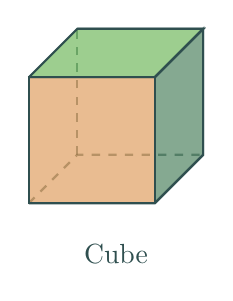
\begin{tikzpicture}[thick,scale=0.8,DarkSlateGray]
    \coordinate (A1) at (-1,-1,-1);
    \coordinate (A2) at (-1,-1,1);
    \coordinate (A3) at (-1,1,-1);
    \coordinate (A4) at (-1,1,1);
    \coordinate (B1) at (1,-1,-1);
    \coordinate (B2) at (1,-1,1);
    \coordinate (B3) at (1,1,-1);
    \coordinate (B4) at (1,1,1);
    % Drawing dashed lines
    \draw[dashed,opacity=0.6] (A2) -- (A1) -- (B1);
    \draw[dashed,opacity=0.6] (A1) -- (A3);
    % Color Faces
    \draw[fill=cof,opacity=0.6]   (A4) -- (B4) -- (B2) -- (A2) ;
    \draw[fill=greet,opacity=0.6]   (B4) -- (B3) -- (B1) -- (B2) ;
    \draw[fill=greeo,opacity=0.6] (A4) -- (B4) -- (B3) -- (A3) ;
    % Drawing Edges
    \draw (A2) -- (B2) -- (B1) ;
    \draw (A2) -- (A4) -- (B4) -- (B2) -- cycle ;
    \draw (A4) -- (A3) -- (B3) -- (B4) ;   
    \draw (B3) -- (B1);
    %
    \node[thick,below=1.5cm] {Cube};
\end{tikzpicture}
% OCTAHEDRON
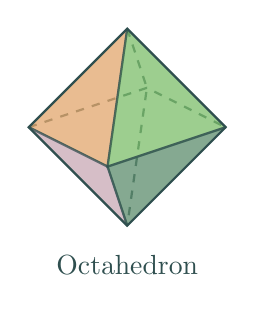
\begin{tikzpicture}[thick,scale=2.5,DarkSlateGray]
    \coordinate (A1) at (0,0);
    \coordinate (A2) at (0.6,0.2);
    \coordinate (A3) at (1,0);
    \coordinate (A4) at (0.4,-0.2);
    \coordinate (B1) at (0.5,0.5);
    \coordinate (B2) at (0.5,-0.5);
    %
    \draw[dashed,opacity=0.6] (A1) -- (A2) -- (A3);        
    \draw[dashed,opacity=0.6] (B1) -- (A2) -- (B2);
    %
    \draw[fill=cof,opacity=0.6] (A1) -- (A4) -- (B1);
    \draw[fill=pur,opacity=0.6] (A1) -- (A4) -- (B2);
    \draw[fill=greeo,opacity=0.6] (A3) -- (A4) -- (B1);
    \draw[fill=greet,opacity=0.6] (A3) -- (A4) -- (B2);
    \draw (B1) -- (A1) -- (B2) -- (A3) --cycle;
    %
    \node[thick,below=1.5cm] at (0.5,0) {Octahedron};
\end{tikzpicture}
% Dodecahedron
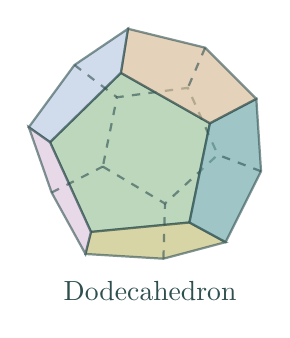
\begin{tikzpicture}[thick,scale=0.5,DarkSlateGray]
    \coordinate (A) at (0,0);
    \coordinate (B) at (2.5,0.24);
    \coordinate (C) at (3.02,2.76);
    \coordinate (D) at (0.76,4.04);
    \coordinate (E) at (-1.04,2.28);
    \coordinate (A1) at (0.3,1.66);
    \coordinate (B1) at (1.88,0.72);
    \coordinate (C1) at (3.22,1.96);
    \coordinate (D1) at (2.46,3.66);
    \coordinate (E1) at (0.66,3.42);
    \coordinate (B2) at (-.14,-.56);
    \coordinate (C2) at (1.84,-.68);
    \coordinate (D2) at (3.42,-.26);
    \coordinate (B3) at (4.32,1.54);
    \coordinate (C3) at (4.2,3.38);
    \coordinate (D3) at (2.9,4.68);
    \coordinate (B4) at (.94,5.16);
    \coordinate (C4) at (-.42,4.24);
    \coordinate (D4) at (-1.58,2.66);
    \coordinate (F) at (-1,1);
    
    \draw[fill=DarkSeaGreen,opacity=0.6] (A)--(B)--(C)--(D)--(E)--cycle;
    \draw[opacity=0.6,dashed] (A1)--(B1)--(C1)--(D1)--(E1)--cycle;
    \draw[fill=DarkKhaki,opacity=0.6] (A)--(B2)--(C2)--(D2)--(B)--cycle;
    \draw[fill=CadetBlue,opacity=0.6] (B)--(D2)--(B3)--(C3)--(C)--cycle;
    \draw[fill=Tan,opacity=0.6] (C)--(C3)--(D3)--(B4)--(D)--cycle;
    \draw[fill=LightSteelBlue,opacity=0.6] (D)--(B4)--(C4)--(D4)--(E)--cycle;
    \draw[fill=Thistle,opacity=0.6] (E)--(D4)--(F)--(B2)--(A)--cycle;
    \path[opacity=0.6] (B2)--(C2)--(B1)--(A1)--(F)--cycle;
    \draw[opacity=0.6,dashed] (C2)--(B1) (F)--(A1);
    \path[opacity=0.6] (C2)--(D2)--(B3)--(C1)--(B1)--cycle;
    \draw[opacity=0.6,dashed] (B3)--(C1);
    \path[opacity=0.6] (B3)--(C3)--(D3)--(D1)--(C1)--cycle;
    \draw[opacity=0.6,dashed] (D3)--(D1);
    \path[opacity=0.6] (D3)--(B4)--(C4)--(E1)--(D1)--cycle;
    \draw[opacity=0.6,dashed] (C4)--(E1);
%titik dengan ball
%http://tex.stackexchange.com/questions/228946/prevent-shifting-of-shading-center-point-when-using-relative-coordinates
    % \shadedraw[ball color=DarkSlateGray!15!white, draw=DarkSlateGray!50] (A) circle (0.08) ;
    % \shadedraw[ball color=DarkSlateGray!15!white, draw=DarkSlateGray!50](B) circle (0.08);
    % \shadedraw[ball color=DarkSlateGray!15!white, draw=DarkSlateGray!50](C) circle (0.08);
    % \shadedraw[ball color=DarkSlateGray!15!white, draw=DarkSlateGray!50](D) circle (0.08);
    % \shadedraw[ball color=DarkSlateGray!15!white, draw=DarkSlateGray!50](E) circle (0.08);
    % \shadedraw[ball color=DarkSlateGray!15!white, draw=DarkSlateGray!50](F) circle (0.08);
    % \shadedraw[ball color=DarkSlateGray!15!white, draw=DarkSlateGray!50] (A1) circle (0.08) ;
    % \shadedraw[ball color=DarkSlateGray!15!white, draw=DarkSlateGray!50](B1) circle (0.08);
    % \shadedraw[ball color=DarkSlateGray!15!white, draw=DarkSlateGray!50](C1) circle (0.08);
    % \shadedraw[ball color=DarkSlateGray!15!white, draw=DarkSlateGray!50](D1) circle (0.08);
    % \shadedraw[ball color=DarkSlateGray!15!white, draw=DarkSlateGray!50](E1) circle (0.08);
    % \shadedraw[ball color=DarkSlateGray!15!white, draw=DarkSlateGray!50](B2) circle (0.08);
    % \shadedraw[ball color=DarkSlateGray!15!white, draw=DarkSlateGray!50](C2) circle (0.08);
    % \shadedraw[ball color=DarkSlateGray!15!white, draw=DarkSlateGray!50](D2) circle (0.08);
    % \shadedraw[ball color=DarkSlateGray!15!white, draw=DarkSlateGray!50](B3) circle (0.08);
    % \shadedraw[ball color=DarkSlateGray!15!white, draw=DarkSlateGray!50](C3) circle (0.08);
    % \shadedraw[ball color=DarkSlateGray!15!white, draw=DarkSlateGray!50](D3) circle (0.08);
    % \shadedraw[ball color=DarkSlateGray!15!white, draw=DarkSlateGray!50](B4) circle (0.081);
    % \shadedraw[ball color=DarkSlateGray!15!white, draw=DarkSlateGray!50](C4) circle (0.08);
    % \shadedraw[ball color=DarkSlateGray!15!white, draw=DarkSlateGray!50](D4) circle (0.08);
   %
    \node[thick,below=0.5cm] at (1.5,0,0) {Dodecahedron};
\end{tikzpicture}
% Icosphedron
    \tdplotsetmaincoords{60}{100}
    \begin{tikzpicture}[tdplot_main_coords,scale=1,line join=round, scale=0.4, DarkSlateGray]
    \pgfmathsetmacro\a{2}
    \pgfmathsetmacro{\phi}{\a*(1+sqrt(5))/2}
    \path 
    coordinate(A) at (0,\phi,\a)
    coordinate(B) at (0,\phi,-\a)
    coordinate(C) at (0,-\phi,\a)
    coordinate(D) at (0,-\phi,-\a)
    coordinate(E) at (\a,0,\phi)
    coordinate(F) at (\a,0,-\phi)
    coordinate(G) at (-\a,0,\phi)
    coordinate(H) at (-\a,0,-\phi)
    coordinate(I) at (\phi,\a,0)
    coordinate(J) at (\phi,-\a,0)
    coordinate(K) at (-\phi,\a,0)
    coordinate(L) at (-\phi,-\a,0); 
    \draw[dashed, thick]    (B) -- (H) -- (F) 
    (D) -- (L) -- (H) --cycle 
    (K) -- (L) -- (H) --cycle
    (K) -- (L) -- (G) --cycle
    (C) -- (L) (B)--(K) (A)--(K)
    ;

        \draw[thick]
        (A) -- (I) -- (B) --cycle 
        (F) -- (I) -- (B) --cycle 
        (F) -- (I) -- (J) --cycle
        (F) -- (D) -- (J) --cycle
        (C) -- (D) -- (J) --cycle
        (C) -- (E) -- (J) --cycle
        (I) -- (E) -- (J) --cycle
        (I) -- (E) -- (A) --cycle
        (G) -- (E) -- (A) --cycle
        (G) -- (E) -- (C) --cycle
        ; 
        \draw[fill=DarkSeaGreen,opacity=0.6] (A) -- (I) -- (B) --cycle ;
        \draw[fill=DarkKhaki,opacity=0.6]  (F) -- (I) -- (B) --cycle ;
        \draw[fill=Tan,opacity=0.6]  (F) -- (I) -- (J) --cycle;
        \draw[fill=CadetBlue,opacity=0.6]  (F) -- (D) -- (J) --cycle;
        \draw[fill=LightYellow,opacity=0.6]    (C) -- (D) -- (J) --cycle;
        \draw[fill=Thistle,opacity=0.6]   (C) -- (E) -- (J) --cycle;
        \draw[fill=DarkGray,opacity=0.6]  (I) -- (E) -- (J) --cycle;
        \draw[fill=LightSteelBlue,opacity=0.6]     (I) -- (E) -- (A) --cycle;
        \draw[fill=DarkSalmon,opacity=0.6]   (G) -- (E) -- (A) --cycle;
        \draw[fill=LightPink,opacity=0.6]    (G) -- (E) -- (C) --cycle;
           %
        \node[thick,below=1.5cm] at (0.7,0,0) {Icosahedron};
\end{tikzpicture}

    \end{figure}
    %
    \begin{itemize}
        \item In this course, we skip platonic solids (except tetrahedron and cube).
    \end{itemize}
\end{frame}
%%%%%%%%%%%%%%%%%%%%%%%%%%%%%%%%%%%%%%%
%        SLIDE 
%%%%%%%%%%%%%%%%%%%%%%%%%%%%%%%%%%%%%%%
\subsection{Prism}
\begin{frame}[t]{Prism}
    \begin{itemize}
        \item Have two faces which are congruent, parallel. These faces are called \textbf{bases}.
        \item All the other faces are called \textbf{lateral faces}. 
        \item Lateral faces can be either:
        \begin{itemize}
            \item parallelogram (oblique prism)
            \item rectangle (right prism)
        \end{itemize}
    \end{itemize}
    %
    \begin{figure}[H]
        \centering
        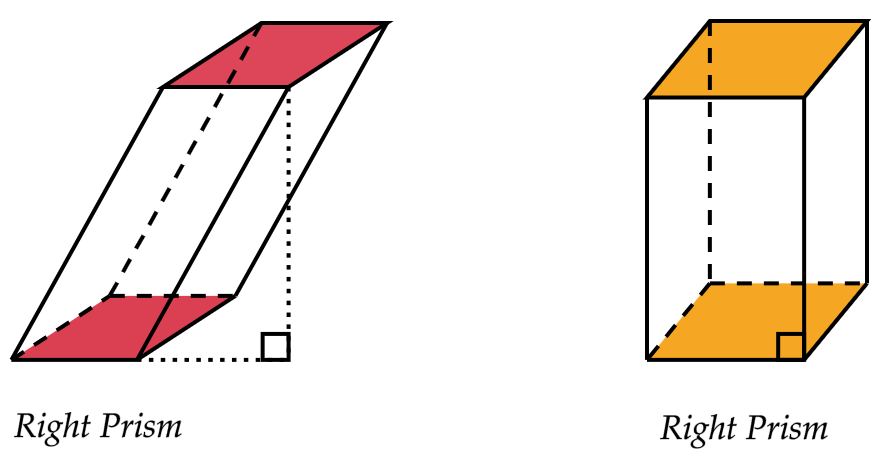
\includegraphics[scale=0.24]{pics/prism.png}
    \end{figure}
    %
    \begin{itemize}
        \item In this course, we only discuss about right prism.
    \end{itemize}
\end{frame}
%%%%%%%%%%%%%%%%%%%%%%%%%%%%%%%%%%%%%%%
%        SLIDE 
%%%%%%%%%%%%%%%%%%%%%%%%%%%%%%%%%%%%%%%
\begin{frame}{Prism (Cont'd)}
    \begin{itemize}
        \item Some examples of right prisms:
    \end{itemize}
    %
    \begin{figure}[H]
        \centering
        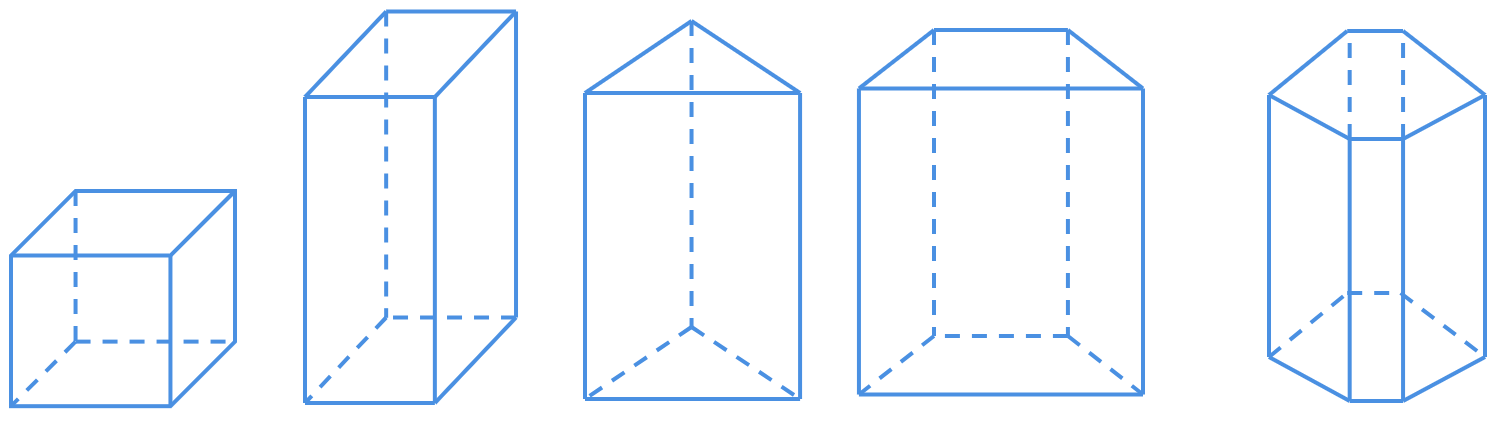
\includegraphics[scale=0.25]{pics/other_prisms.png}
    \end{figure}
\end{frame}
%%%%%%%%%%%%%%%%%%%%%%%%%%%%%%%%%%%%%%%
%        SLIDE 
%%%%%%%%%%%%%%%%%%%%%%%%%%%%%%%%%%%%%%%
\subsection{Pyramid}
\begin{frame}[t]{Pyramid}
    \begin{itemize}
        \item All faces except one intersect at a common vertex.
        \item It has only one base.
    \end{itemize}
    %
    \begin{figure}[H]
        \centering
        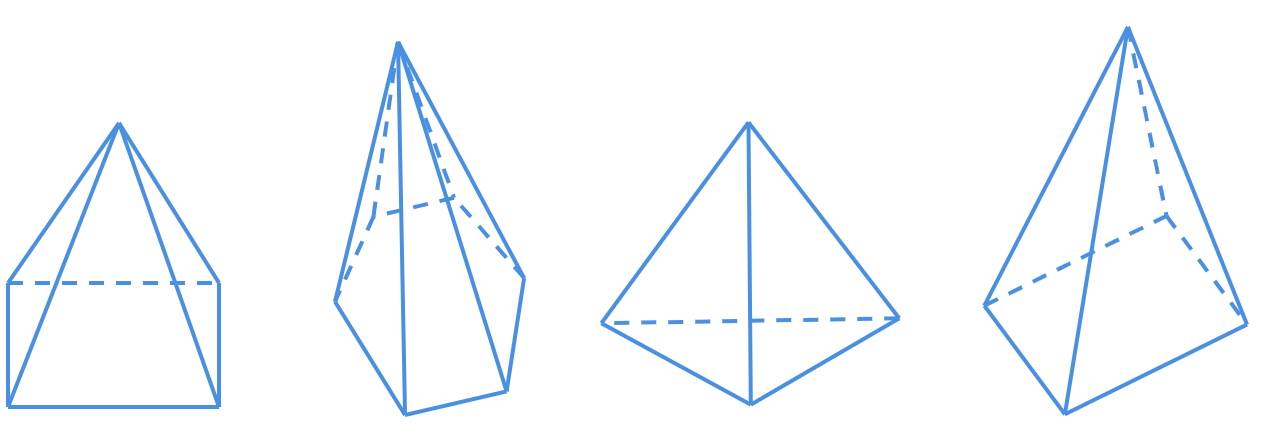
\includegraphics[scale=0.26]{pics/pyramids.png}
    \end{figure}
\end{frame}
%%%%%%%%%%%%%%%%%%%%%%%%%%%%%%%%%%%%%%%
%        SLIDE 
%%%%%%%%%%%%%%%%%%%%%%%%%%%%%%%%%%%%%%%
\section{Volume and Surface Area}
\begin{frame}[t]{Volume and Surface Area}
    \begin{columns}[t]
    \column{0.45\textwidth}
    %
    \boxed{\textbf{Surface Area (SA)}}
    \begin{itemize}
        \item The sum of the areas of all of the faces of a polyhedron.
        \item Surface Area is denoted as SA.
    \end{itemize}
    %
    \begin{figure}[H]
        \centering
        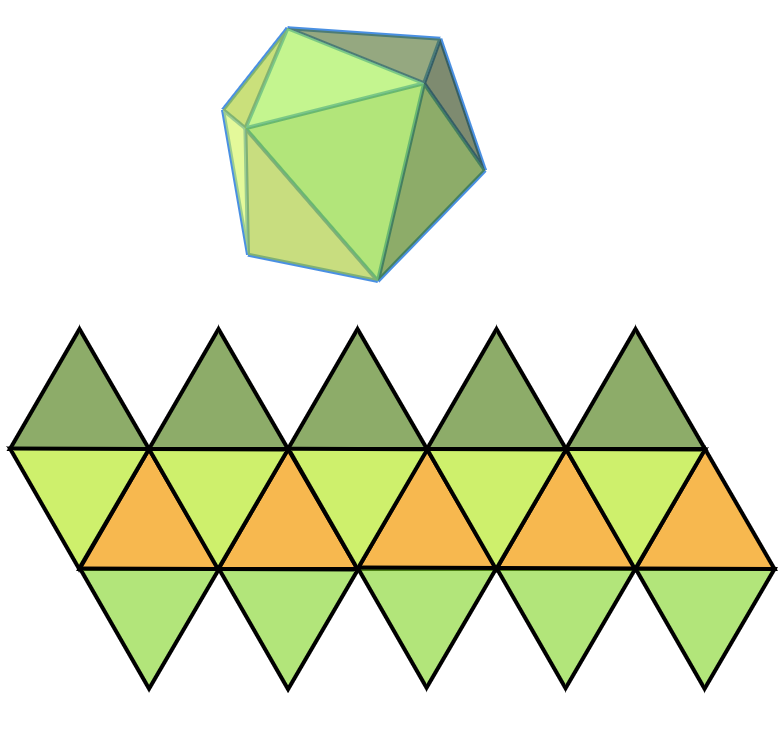
\includegraphics[scale=0.17]{pics/def_surface_area.png}
    \end{figure}
    %
    \column{0.45\textwidth}
    %    
    \boxed{\textbf{Volume ($V$)}}
        \begin{itemize}
            \item The amount of space inside of a shape.
            \item Volume is measured by cubic units. 
        \end{itemize}
    %
    \begin{figure}[H]
        \centering
        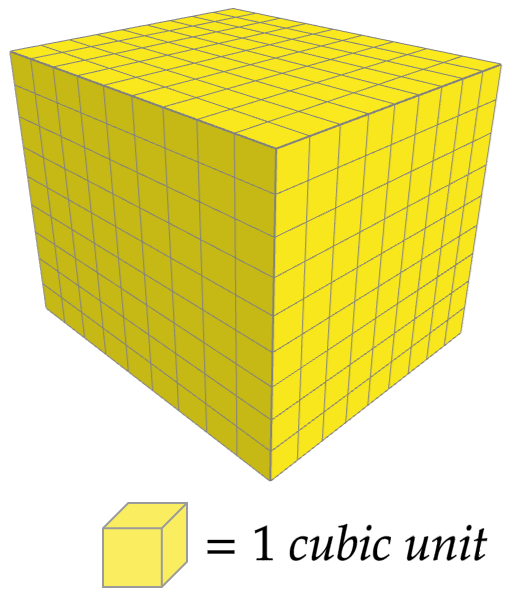
\includegraphics[scale=0.17]{pics/def_volume.png}
    \end{figure}
    %
    \end{columns}
\end{frame}
%%%%%%%%%%%%%%%%%%%%%%%%%%%%%%%%%%%%%%%
%        SLIDE 
%%%%%%%%%%%%%%%%%%%%%%%%%%%%%%%%%%%%%%%
\subsection{Volume and SA of a Prism}
\begin{frame}[t]{Volume and SA of a Prism}
    %
    \begin{columns}[t]
    % SA
    \column{0.45\textwidth}
    \textbf{Surface Area (SA)}
    \begin{itemize}
        \item To find the SA of a prism, you just need to find the area of all faces and add them together.
        \item In this course, we mainly focus on volume of the prism.
    \end{itemize}
    % Volume
    \column{0.45\textwidth}
    \textbf{Volume ($V$)}
    \begin{block}{Formula}
         \[ V = B\cdot h \]
         where $B$ is the area of one base and $h$ is the distance between two bases.
    \end{block}
    \end{columns}
    %
\begin{figure}[H]
    \centering
    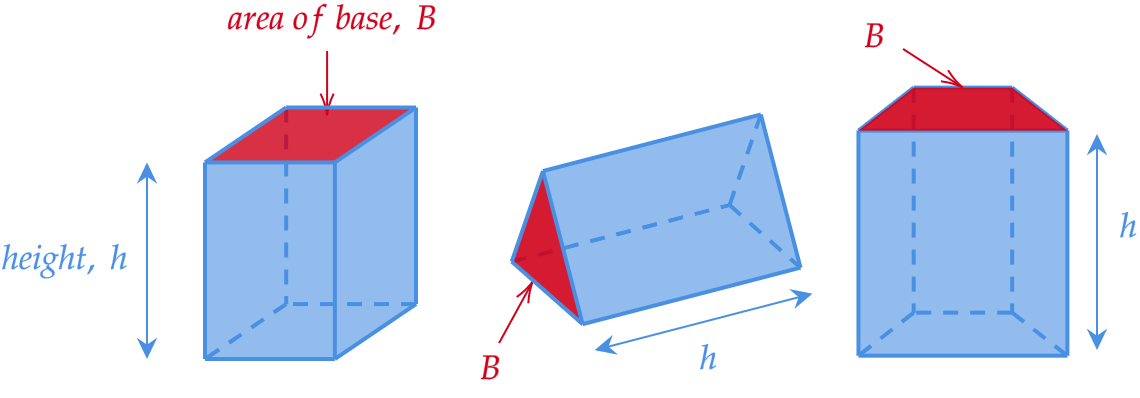
\includegraphics[scale=0.25]{pics/volume_of_prism.png}
\end{figure}
\end{frame}
%%%%%%%%%%%%%%%%%%%%%%%%%%%%%%%%%%%%%%%
%        SLIDE 
%%%%%%%%%%%%%%%%%%%%%%%%%%%%%%%%%%%%%%%
\begin{frame}[t]{Example (Prism)}
    \begin{columns}
        \column{0.45\textwidth}
        \begin{example}
            Find the volume of the prism on the right.
        \end{example}
        %
        \column{0.45\textwidth}
        \begin{figure}[H]
            \centering
            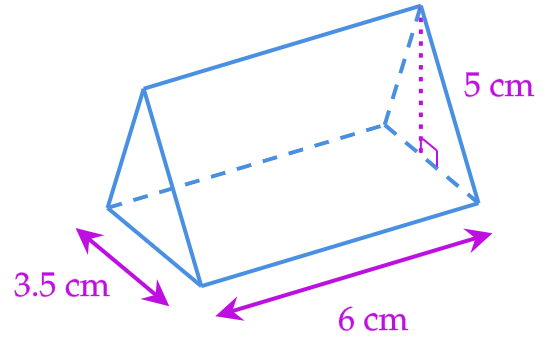
\includegraphics[scale=0.25]{pics/example_volume_prism.png}
        \end{figure}
    \end{columns}
\end{frame}
%%%%%%%%%%%%%%%%%%%%%%%%%%%%%%%%%%%%%%%
%        SLIDE 
%%%%%%%%%%%%%%%%%%%%%%%%%%%%%%%%%%%%%%%
\subsection{Volume and SA of a Pyramid}
\begin{frame}[t]{Volume and SA of a Pyramid}
    %
    \begin{columns}[t]
    % SA
    \column{0.45\textwidth}
    \textbf{Surface Area (SA)}
    \begin{itemize}
        \item Similar to prism, to find SA of a pyramid, just add up the areas of all faces.
        \item In this course, we will work on its volume.
    \end{itemize}
    % Volume
    \column{0.45\textwidth}
    \textbf{Volume ($V$)}
    \begin{block}{Formula}
         \[ V = \frac{B\cdot h}{3} \]
         where $B$ is the area of a base and $h$ is the distance from the common vertex to base.
    \end{block}
    \end{columns}
    %
\begin{figure}[H]
    \centering
    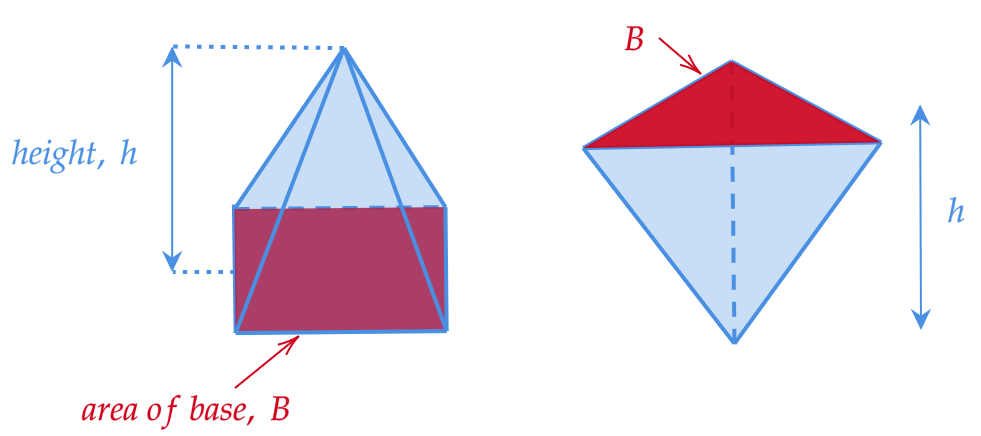
\includegraphics[scale=0.22]{pics/volume_of_pyramid.png}
\end{figure}
\end{frame}
%%%%%%%%%%%%%%%%%%%%%%%%%%%%%%%%%%%%%%%
%        SLIDE 
%%%%%%%%%%%%%%%%%%%%%%%%%%%%%%%%%%%%%%%
\begin{frame}[t]{Example (Pyramid}
    \begin{columns}[c]
        \column{0.45\textwidth}
        \begin{example}
            Find the volume of the pyramid on the right.
        \end{example}
        %
        \column{0.45\textwidth}
        \begin{figure}[H]
            \centering
            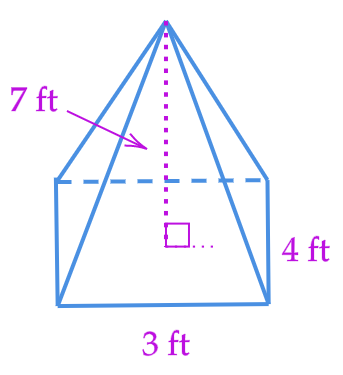
\includegraphics[scale=0.25]{pics/example_volume_pyramid.png}
        \end{figure}
    \end{columns}    
\end{frame}
%%%%%%%%%%%%%%%%%%%%%%%%%%%%%%%%%%%%%%%
%        SLIDE 
%%%%%%%%%%%%%%%%%%%%%%%%%%%%%%%%%%%%%%%
\subsection{Volume and SA of a Rectangular Cube}
\begin{frame}[t]{Volume and SA of a Rectangular Cube (Box)}
    %
    \begin{columns}[t]
    % SA
    \column{0.45\textwidth}
    \textbf{Surface Area (SA)}
    \begin{itemize}
        \item SA can be found easily by opening the box and looking at each face.
    \end{itemize}
    %
    \begin{block}{SA Formula}
         \[ SA = 2\ell w+ 2\ell h+ 2wh \]
    \end{block}
    %
    \begin{figure}[H]
        \centering
        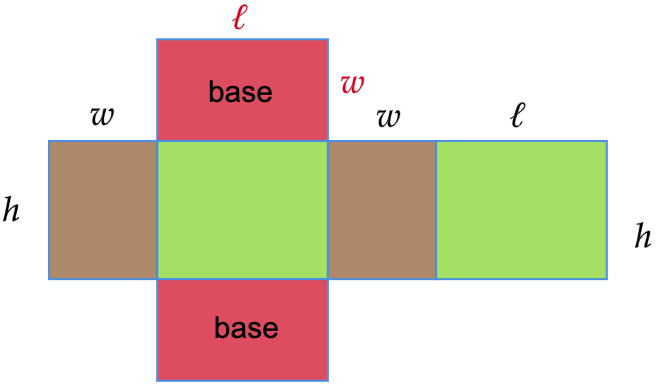
\includegraphics[scale=0.22]{pics/box_SA.png}
    \end{figure}
    % Volume
    \column{0.45\textwidth}
    \textbf{Volume ($V$)}
    %
    \begin{itemize}
        \item We can easily find its volume since it is a prism.
    \end{itemize}
    %
    \begin{block}{Volume Formula}
         \[ V = \ell w h \]
    \end{block}
    %
    \begin{figure}[H]
        \centering
        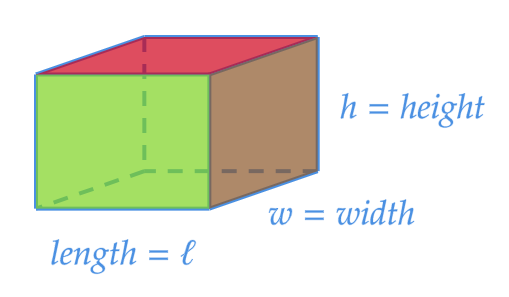
\includegraphics[scale=0.29]{pics/box_volume.png}
    \end{figure}
    \end{columns}
\end{frame}
%%%%%%%%%%%%%%%%%%%%%%%%%%%%%%%%%%%%%%%
%        SLIDE 
%%%%%%%%%%%%%%%%%%%%%%%%%%%%%%%%%%%%%%%
\subsection{Volume and SA of a Cube}
\begin{frame}[t]{Volume and SA of a Cube}
    %
    \begin{columns}[t]
    % SA
    \column{0.45\textwidth}
    \textbf{Surface Area (SA)}
    \begin{itemize}
        \item Cube is a rectangular box in which all sides are equal to $s$.
    \end{itemize}
    %
    \begin{block}{SA Formula}
         \[ SA = 6s^2\]
    \end{block}
    %
    % Volume
    \column{0.45\textwidth}
    \textbf{Volume ($V$)}
    %
    \begin{itemize}
        \item Similar to SA, use the box formula and replace all sides with $s$.
    \end{itemize}
    %
    \begin{block}{Volume Formula}
         \[ V = s^3 \]
    \end{block}
    %
    \end{columns}
    %
    \begin{figure}[H]
        \centering
        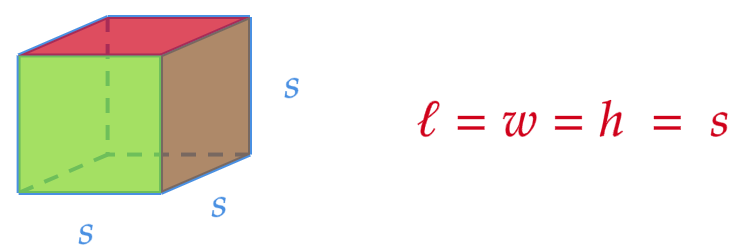
\includegraphics[scale=0.28]{pics/cube_volume.png}
    \end{figure}
\end{frame}
%%%%%%%%%%%%%%%%%%%%%%%%%%%%%%%%%%%%%%%
%        SLIDE 
%%%%%%%%%%%%%%%%%%%%%%%%%%%%%%%%%%%%%%%
\begin{frame}[t]{Example (Cube and Box)}
    \begin{columns}[t]
    %
    \column{0.45\textwidth}
    \begin{example}
        Find the SA and volume of the shapes on the right.
    \end{example}
    %
    \column{0.45\textwidth}
    \begin{figure}[H]
        \centering
        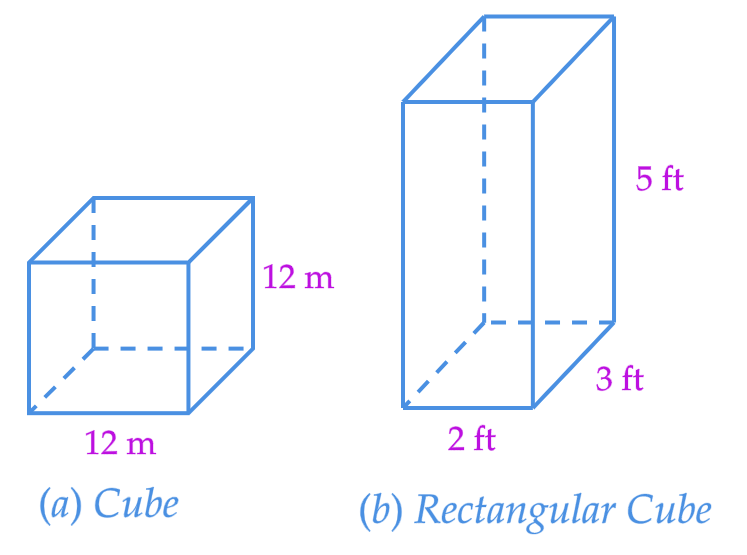
\includegraphics[scale=0.2]{pics/example_cube_box.png}
    \end{figure}
    \end{columns}
\end{frame}
%%%%%%%%%%%%%%%%%%%%%%%%%%%%%%%%%%%%%%%
%        SLIDE 
%%%%%%%%%%%%%%%%%%%%%%%%%%%%%%%%%%%%%%%
\section{Non-Polyhedra Shapes}
\begin{frame}[t]{Non-Polyhedra Shapes}
    \begin{itemize}
        \item We will discuss three shapes that are not polyhedra:
        \begin{itemize}
            \item Cylinder
            \item Cone
            \item Sphere
        \end{itemize}
    \end{itemize}
    %
    \begin{itemize}
        \item Their SA is little bit complicated than polyhedra!
        \item The volume of Cylinder and Cone is like Prim and Pyramid, respectively.
        \item However, the volume of sphere is totally different.
    \end{itemize}
    %
    \begin{figure}[H]
        \centering
        %%%%%%%%%%%%%%%%%%%%
%  Sphere
%%%%%%%%%%%%%%%%%%%%
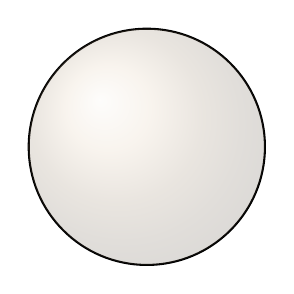
\begin{tikzpicture}[scale=1.5]
    %\draw (-1,0) arc (180:360:1cm and 0.5cm);
    %\draw[dashed] (-1,0) arc (180:0:1cm and 0.5cm);
    %\draw (0,1) arc (90:270:0.5cm and 1cm);
    %\draw[dashed] (0,1) arc (90:-90:0.5cm and 1cm);
    \draw (0,0) circle (1cm);
    \shade[ball color=Tan, opacity=0.20] (0,0) circle (1cm);
\end{tikzpicture}
\hspace{1em}
%%%%%%%%%%%%%%%%%%%%
%  Cone
%%%%%%%%%%%%%%%%%%%%
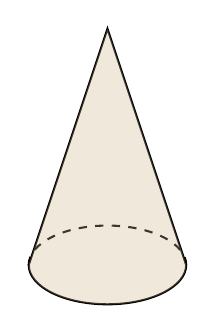
\begin{tikzpicture}
    \draw (-1,0) arc (180:360:1cm and 0.5cm) -- (0,3) -- cycle;
    \draw[dashed] (-1,0) arc (180:0:1cm and 0.5cm);
    \shade[left color=Tan,right color=Tan,opacity=0.3] (-1,0) arc (180:360:1cm and 0.5cm) -- (0,3) -- cycle;
\end{tikzpicture}
%%%%%%%%%%%%%%%%%%%%
\hspace{1em}
%%%%%%%%%%%%%%%%%%%%
%  Cylinder
%%%%%%%%%%%%%%%%%%%%
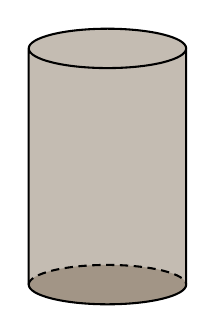
\begin{tikzpicture}[scale=0.5]
    \fill[top color=Tan,bottom color=Tan,middle color=Tan,shading=axis,opacity=0.25] (0,0) circle (2cm and 0.5cm);
    \fill[left color=Tan, right color=Tan,middle color=Tan,shading=axis,opacity=0.25] (2,0) -- (2,6) arc (360:180:2cm and 0.5cm) -- (-2,0) arc (180:360:2cm and 0.5cm);
    \fill[top color=Tan,bottom color=Tan,middle color=Tan,shading=axis,opacity=0.25] (0,6) circle (2cm and 0.5cm);
    \draw (-2,6) -- (-2,0) arc (180:360:2cm and 0.5cm) -- (2,6) ++ (-2,0) circle (2cm and 0.5cm);
    \draw[densely dashed] (-2,0) arc (180:0:2cm and 0.5cm);
\end{tikzpicture}
    \end{figure}
\end{frame}


%%%%%%%%%%%%%%%%%%%%%%%%%%%%%%%%%%%%%%%
%        SLIDE 
%%%%%%%%%%%%%%%%%%%%%%%%%%%%%%%%%%%%%%%
\subsection{Volume and SA of a Cylinder (Right Cylinder)}
\begin{frame}[t]{Volume and SA of a Cylinder}
    \begin{columns}[t]
    % SA
    \column{0.45\textwidth}
    \textbf{Surface Area (SA)}
    \begin{itemize}
        \item The bases of a cylinder are circles.
        \item The area of a lateral face can be found by cutting the cylinder.
    \end{itemize}
    %
    \begin{block}{SA Formula}
         \[ SA = 2\pi r^2 + 2\pi rh\]
    \end{block}
    %
    \begin{figure}[H]
        \centering
        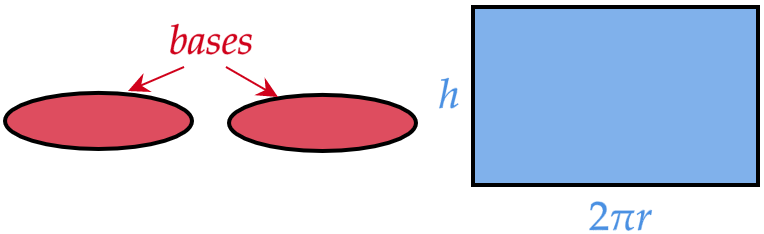
\includegraphics[scale=0.252]{pics/cylinder_SA.png}
    \end{figure}
    % Volume
    \column{0.45\textwidth}
    \textbf{Volume ($V$)}
    %
    \begin{itemize}
        \item Similar to prism, the volume of cylinder is area of a base ($\pi r^2$) times $h$ (distance between two bases).
    \end{itemize}
    %
    \begin{block}{Volume Formula}
         \[ V = \pi r^2 h \]
    \end{block}
    %
    \begin{figure}[H]
        \centering
        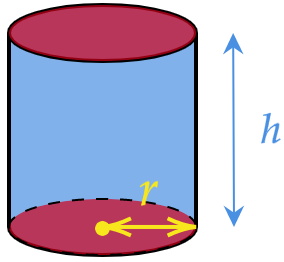
\includegraphics[scale=0.27]{pics/cylinder_v.png}
    \end{figure}
    \end{columns}
    %
\end{frame}
%%%%%%%%%%%%%%%%%%%%%%%%%%%%%%%%%%%%%%%
%        SLIDE 
%%%%%%%%%%%%%%%%%%%%%%%%%%%%%%%%%%%%%%%
\begin{frame}[t]{Example (Cylinder)}
    \begin{columns}[t]
        \column{0.45\textwidth}
        \begin{example}
            Find the surface area and volume of the following cylinder.
        \end{example}
        %
        \column{0.45\textwidth}
        \begin{figure}[H]
            \centering
            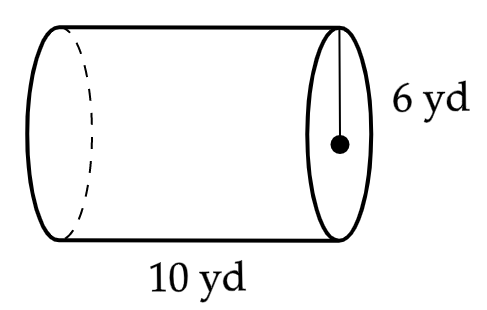
\includegraphics[scale=0.3]{pics/example_cylinder.png}
        \end{figure}
    \end{columns}
\end{frame}
%%%%%%%%%%%%%%%%%%%%%%%%%%%%%%%%%%%%%%%
%        SLIDE 
%%%%%%%%%%%%%%%%%%%%%%%%%%%%%%%%%%%%%%%
\subsection{Volume and SA of a Cone}
\begin{frame}[t]{Volume and SA of a Cone}
    \begin{columns}[t]
    % SA
    \column{0.45\textwidth}
    \textbf{Surface Area (SA)}
    \begin{itemize}
        \item The base of the cone is a circle.
        \item If we cut the cone and open it, we can find its lateral face area.
    \end{itemize}
    %
    \begin{block}{SA Formula}
         \[ SA = \pi r^2 + \pi r \sqrt{r^2+h^2}\]
    \end{block}
    %
    \begin{figure}[H]
        \centering
        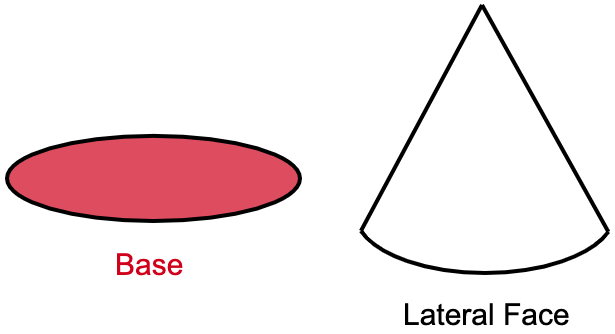
\includegraphics[scale=0.23]{pics/cone_SA.png}
    \end{figure}
    % Volume
    \column{0.45\textwidth}
    \textbf{Volume ($V$)}
    %
    \begin{itemize}
        \item Like pyramid, the volume of cone is one third of the volume of the cylinder with
        same height and radius.
    \end{itemize}
    %
    \begin{block}{Volume Formula}
         \[ V = \frac{\pi r^2 h}{3} \]
    \end{block}
    %
    \begin{figure}[H]
        \centering
        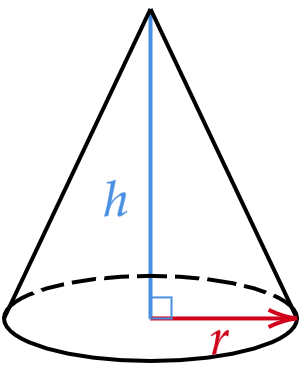
\includegraphics[scale=0.18]{pics/cone_v.png}
    \end{figure}
    \end{columns}
    %
\end{frame}
%%%%%%%%%%%%%%%%%%%%%%%%%%%%%%%%%%%%%%%
%        SLIDE 
%%%%%%%%%%%%%%%%%%%%%%%%%%%%%%%%%%%%%%%
\begin{frame}[t]{Example (Cone)}
    \begin{columns}[t]
    \column{0.45\textwidth}
        \begin{example}
            Find the SA and volume of the following cone.
        \end{example}
    \column{0.45\textwidth}
        \begin{figure}[H]
            \centering
            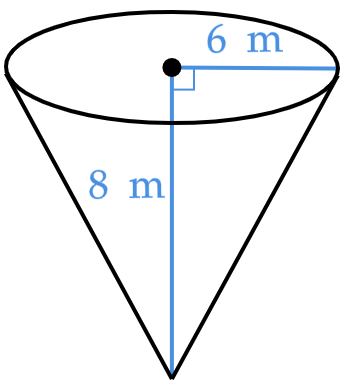
\includegraphics[scale=0.25]{pics/example_cone.png}
        \end{figure}
    \end{columns}
\end{frame}
%%%%%%%%%%%%%%%%%%%%%%%%%%%%%%%%%%%%%%%
%        SLIDE 
%%%%%%%%%%%%%%%%%%%%%%%%%%%%%%%%%%%%%%%
\subsection{Volume and SA of a Sphere}
\begin{frame}[t]{Volume and SA of a Sphere}
    \begin{columns}[t]
    % SA
    \column{0.5\textwidth}
    \footnotesize{
    \begin{itemize}
        \item Archimedes was the first person who discovered the SA and volume of a sphere.
        \item Fitted a cylinder around a sphere.
        \item Cut horizontal slices through the cylinder.
        \item Found the volume between cylinder and sphere.
        \item Then he found the volume of sphere.
        \item Similar technique used to find the SA.
    \end{itemize}}
    %
    \begin{figure}[H]
        \centering
        \input{Tikz/sphere}
    \end{figure}
    \column{0.45\textwidth}
    %
    \begin{block}{SA and Volume Formula}
         \begin{align*}
             SA & = 4 \pi r^2
             \\
             V & = \frac{4\pi r^3}{3}
         \end{align*}
    \end{block}
    %
    \begin{figure}[H]
        \centering
        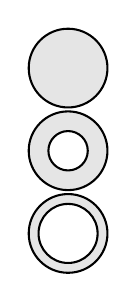
\begin{tikzpicture}[scale=0.5]
    \tikzset{
      reversed with radius/.style={
        x radius=#1,
        y radius=-#1,
     }
    }
    \draw[preaction={fill,opacity=0.1}] (0,0)
      circle[reversed with radius=1cm]
      circle[radius=0.75cm];
     %
     \draw[preaction={fill,opacity=0.1}] (0,2.1)
      circle[reversed with radius=1cm]
      circle[radius=0.5cm];
    %
    \draw[preaction={fill,opacity=0.1}] (0,4.2)
      circle[reversed with radius=1cm];
\end{tikzpicture}
%
%
%%%%%%%%%%%%%%%%%%%%%
% Sphere and Cylinder
%%%%%%%%%%%%%%%%%%%%%
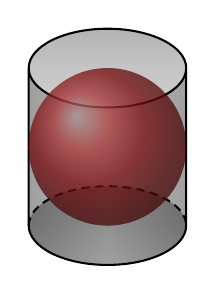
\begin{tikzpicture}
\def\R{1}
  \fill[top color    = gray!50!black,
        bottom color = gray!10,
        middle color = gray,
        shading      = axis,
        opacity      = 0.25]
    (0,0) circle (\R cm and 0.5cm);
  \fill[left color   = gray!50!black,
        right color  = gray!50!black,
        middle color = gray!50,
        shading      = axis,
        opacity      = 0.25]
    (\R,0) -- (\R,2*\R)  arc (360:180:\R cm and 0.5cm)
          -- (-\R,0) arc (180:360:\R cm and 0.5cm);
  \fill[top color    = gray!90!,
        bottom color = gray!2,
        middle color = gray!30,
        shading      = axis,
        opacity      = 0.25]
    (0,2*\R) circle (\R cm and 0.5cm);
  
  \draw (-\R,2*\R) -- (-\R,0) arc (180:360:\R cm and 0.5cm)
              -- (\R,2*\R) ++ (-\R,0) circle (\R cm and 0.5cm);
  \draw[densely dashed] (-\R,0) arc (180:0:\R cm and 0.5cm);
 \fill[thick, ball color=red!90, opacity = 0.5] (0,\R) circle (\R);
% \fill[thick, ball color=orange!90, opacity = 0.5] (0,3*\R) circle (\R);
% \fill[thick, ball color=blue!90, opacity = 0.5] (0,5*\R) circle (\R);
 \end{tikzpicture}
    \end{figure}
    \end{columns}
    %
\end{frame}
%%%%%%%%%%%%%%%%%%%%%%%%%%%%%%%%%%%%%%%
%        SLIDE 
%%%%%%%%%%%%%%%%%%%%%%%%%%%%%%%%%%%%%%%
\begin{frame}[t]{Example (Sphere)}
    \begin{columns}[t]
    \column{0.45\textwidth}
        \begin{example}
            Find the surface area and volume of the golf ball on the right.
        \end{example}
        %
    \column{0.45\textwidth}    
        \begin{figure}[H]
            \centering
            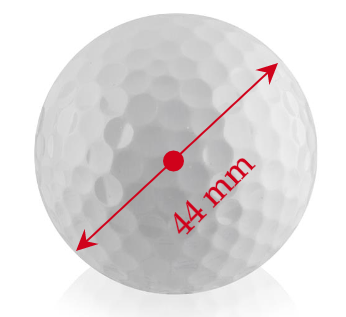
\includegraphics[scale=0.3]{pics/example_golf_ball.png}
        \end{figure}
    \end{columns}
\end{frame}


